\documentclass[a4paper, 12pt]{article}

\usepackage[T1]{fontenc}
\usepackage{IEEEtrantools}
\usepackage[]{amsmath}
\usepackage{amssymb}
\usepackage{float}
\usepackage[]{graphicx}
\usepackage{subfig}
\usepackage{caption}

\title{Control Systems: Practical 4}
\author{Ruan de Bruyn \and 216054484 \and Quintin Kruger \and 216008466}

\begin{document}

\pagenumbering{gobble}
\maketitle
\newpage
\pagenumbering{roman}
\tableofcontents
\listoffigures
\newpage
\pagenumbering{arabic}

\section{Question 1} % (fold)
\label{sec:question_1}
The purpose of this question is to 

% section question_1 (end)

\section{Question 2}

\begin{figure}[H]
	\centering
	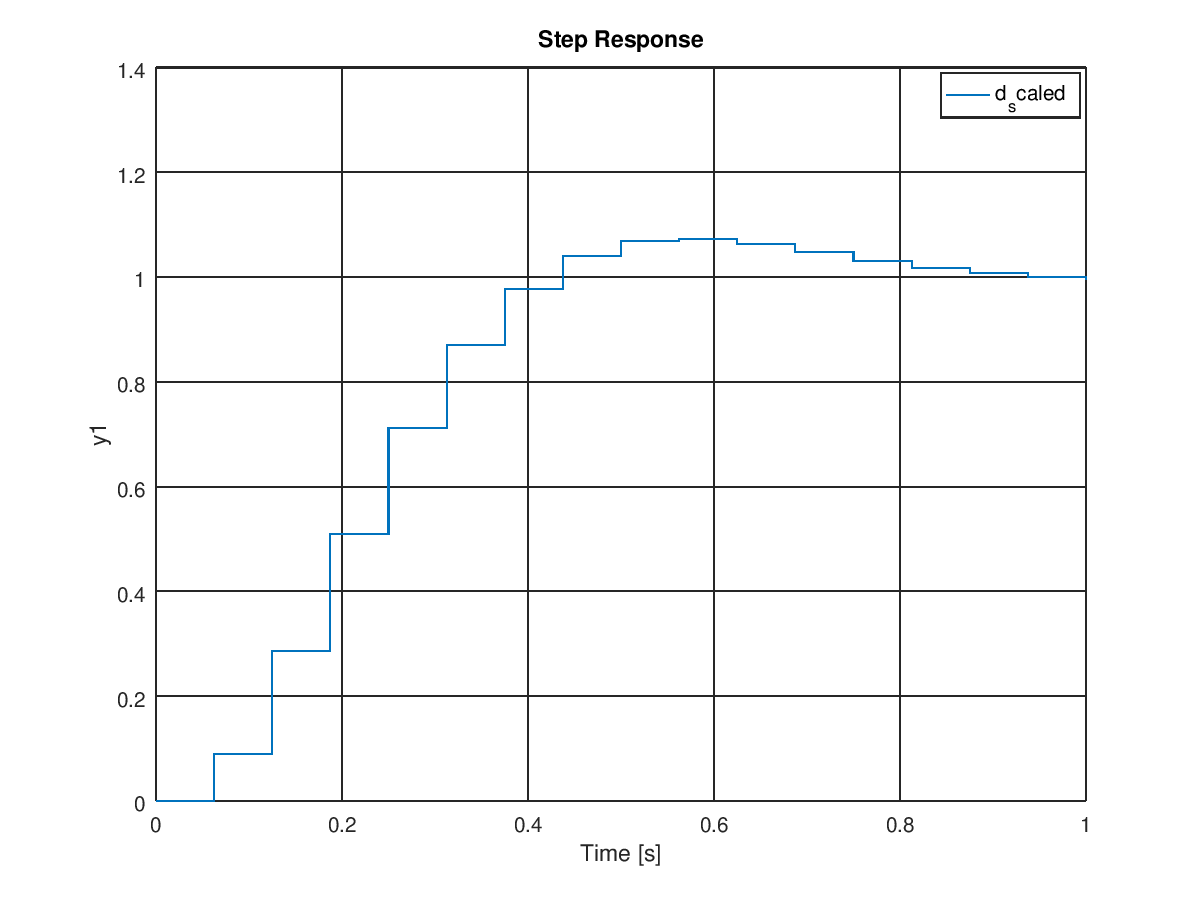
\includegraphics{./img/2_1.png}
	\caption{ZOH system}
	\label{fig:2_1}
\end{figure}

Pole locations: -5 += 6j
Sampling time = 0.6s

% section question_2 (end)
\end{document}
